\documentclass[12pt]{report}
\usepackage{titlesec}
\usepackage{graphicx}
\usepackage{amsmath}
\usepackage{algorithm}
\usepackage{algorithmic}

\usepackage{amssymb}
\graphicspath{{pictures/}}
\DeclareGraphicsExtensions{.pdf,.png,.jpg}
\usepackage{cmap} 
\usepackage[T2A]{fontenc} 
\usepackage[utf8]{inputenc} 
\usepackage[english, ukrainian]{babel} 
\textheight=24cm 
\textwidth=16cm 
\oddsidemargin=0pt 
\topmargin=-2.5cm
\parindent=24pt 
\parskip=0pt 
\tolerance=2000 
\flushbottom 



\begin{document}
\begin{titlepage}
\begin{center}
{\Large Міністерство освіти і науки України\\}
\large  {Львівський національний університет\\імені Івана Франка\\ Кафедра обчислювальної математики}\\
\end{center}
\vspace*{3cm}
\begin{center}

\Large{\textbf{Курсова робота}}\\
\large{На тему}\\
\Large{\textbf{Ієрархічні матриці у методі
		 граничних елементів}}
\end{center}
\normalsize
\vspace*{4cm}\hspace*{8cm}Студентки 4-го курсу групи ПмП-41 \\
\hspace*{8cm}спеціальності \\
\hspace*{8cm}6.040301 "Прикладна матиматика"\\
\hspace*{8cm}Солук О.О.\\

\hspace*{7.1cm}Керівник\\
\hspace*{8cm}Вавричук В.Г.\\
 \\
\hspace*{8cm}\small{Національна шкала} $\underline{ \quad \quad \quad \quad \quad}$\\
\hspace*{8cm}\small{Кількість балів} $\underline{ \quad \quad\quad}$ \small{Оцінка ECTS} $\underline{ \quad \quad \quad}$\\
 \\
\hspace*{4.4cm}\normalsize{Члени комісії}\hspace*{1cm}$\underline{ \quad \quad \quad \quad \quad}$\hspace*{0.5cm}$\underline{ \quad \quad \quad \quad \quad\quad \quad\quad \quad}$\\
\hspace*{8cm}$\underline{ \quad \quad \quad \quad \quad}$\hspace*{0.5cm}$\underline{ \quad \quad \quad \quad \quad\quad \quad\quad \quad}$\\
\hspace*{8cm}$\underline{ \quad \quad \quad \quad \quad}$\hspace*{0.5cm}$\underline{ \quad \quad \quad \quad \quad\quad \quad\quad \quad}$\\
\vspace*{2.5cm}\\
\begin{center}
Львів - 2018
\end{center}
\end{titlepage}
\newpage
	\tableofcontents
\titleformat
{\chapter}[display]
{\bf\Large}{}
{0.5ex}
{
	\vspace{-0.5ex}
}[\vspace{-0.5ex}]
\newpage
\chapter{1. Вступ.}
	\hspace{0.8cm} Ієрархічна матриця ($\mathcal{H}$-матриця) використовується для апроксимації розрідженими даними щільних матриць. Ці матриці застосовують коли намагаються розв'язати систему лінійних рівнянь
	
	 $$ Ax=b \quad\quad  A \in \mathbb{R}^{n\times n} ,\quad   x\in \mathbb{R}^n$$ \newline
	 з майже лінійною складністю $O(n\log(n))$.
	 \par Вперше концепцію ієрахічних матриць запропонував Вольфганг Хакбуш  в 1998 році. Вiн розширив iдею panel clustering methods, зробивши її застосовною до загальних алгебраїчних операцій над матрицями, оберненими матрицями тощо.
	 \par В цій роботі розглянуто базові означення та процес побудови $\mathcal{H}$-матриць, їх застосування на прикладі одновимірної модельної задачі, для розв'язування якої використовують метод граничних елементів (BEM - boundary element method).
	 \par Текст цієї роботи написано на основі матеріалів \cite{HM},\cite{Diss}. Також, деякі графічні ілюстрації взяті з роботи \cite{HM}.
	 \par Автору даної курсової роботи належить власна програмна реалізація на мові С$\#$ таких описаних у роботі алгоритмів:
	 \begin{itemize}
	 	\item побудова cluster tree для $n=2^p$.
	 	\item побудова block cluster tree.
	 	\item множення $\mathcal{H}-$матриці на вектор.
	 	\item реалізація методу спряжених градієнтів.
	 \end{itemize} 
	
\newpage
\chapter{2. Обчислення за допомогою ієрархічних матриць.}
	\section{Означення кластерного дерева.}
	\newtheorem{Def}{Означення}[chapter]
	\begin{Def}
	{\bf (Дерево)} Нехай $V$ - непорожня множина і $E\subseteq V\times V$ є бінарним відношенням над $V$. Пара $\mathbb{T}=(V,E)$, де множина $V=V(\mathbb{T})$ є множиною вершин $\mathbb{T}$, а множина $E=E(\mathbb{T})$ - множина ребер $\mathbb{T}$, називається деревом, якщо виконуються такі умови:
	\begin{enumerate}
		\item[-] Унікальна вершина $v\in V$ називається коренем дерева і позначається $root(\mathbb{T})$ $\Leftrightarrow \forall w\in V:w\not=v$ виконується $(w,v)\not\in E$.
		\item[-] Для будь-якої вершини $v\in V\backslash root(\mathbb{T})$ існує єдиний простий шлях з $root(\mathbb{T})$ до $v$.
	\end{enumerate}

	\end{Def}
	Іншими словами, дерево - це неорієнтований зв'язний граф без простих циклів.
	\par Введемо такі позначення:
	\begin{enumerate}
		\item[$\bullet$] Для вершини $v\in V$ множина її синів визначається як $$S(v)=\{w\in V |(v,w)\in E \}$$
		\item[$\bullet$] Множину всіх листків дерева $\mathbb{T}$ визначають як $\mathcal{L}(\mathbb{T})=\{v\in V|S(v)=\O \}$
		\item[$\bullet$] Рівень дерева $\mathbb{T}$ визначається рекурсивно як $$\mathbb{T}^{(0)}=root(\mathbb{T})$$
		$$\mathbb{T}^{(l)}=\{v \in V|\exists w\in \mathbb{T}^{(l-1)}:(w,v)\in E\}$$
		\item[$\bullet$] Висотою дерева $d(\mathbb{T})$ називається найдовший простий шлях від кореня до листка.
	\end{enumerate}
	
	\hspace{0.8cm}Як $I={0,1...n-1}$ позначемо скінченну множину індексів з потужністю $|I|=n$. В майбутньому, в ролі $I$ використовуватимемо індекси базових функцій, отриманих для дискретизації з методу граничних елементів.
	\begin{Def}
	 {\bf (Кластерне дерево)} Дерево $\mathbb{T}_{I}$ називається кластерним деревом над множиною індексів $I$ з $root(\mathbb{T}_{I})=I$, якщо наступні умови виконуються:
	\begin{enumerate}
		\item[-] $I \in V$ є коренем $\mathbb{T}_{I}$ i $\forall v \in V,v\not=\O \Rightarrow v\subseteq I$.
		\item[-] Якщо $v\in V$ не є листком ($S(v)\not=\O$), то він рівний об'єднанню своїх синів, тобто $v=\bigcup_{w\in S(v)}w$.
	\end{enumerate}
	\end{Def}
	\par $v\in V$ називають кластером.
	\par В одновимірному випадку кластерне деревр - збалансоване бінарне дерево.
	\par {\bf Приклад.} Одновимірний випадок.\newline
	Як корінь дерева $\mathbb{T}_{I}$ беремо множину індексів $I_0^{(0)}=\{0,...,n-1\}$. Для легкості презентації припустимо, що кількість базисних функцій $n$ є степенем 2:
	$$n=2^p$$ 
	\par Розглядаємо випадок, коли $p=3$.Починаючи з кореня, де тільки один кластер, це дерево конструюється шляхом поділу кожної множини індексів $I_i^{(j)}$ на два нащадки $I_{2i}^{(j+1)}$ і $I_{2i+1}^{(j+1)}$ при $0\le i,j\le p$. Нарешті на рівні $p$ всі кластери (вузли) є листками, наприклад $\mathcal{L}(\mathbb{T})=\{I_i^{(3)}\}_{i=0}^7$. Кожен вузол (окрім листків) отриманого дерева матиме рівно два нащадки:
	\par Два нащадки $I_0^{(0)}$: $I_0^{(1)}=\{0,...,\frac{n}{2}-1\}$  i  $I_1^{(1)}=\{\frac{n}{2},...,n-1\}$. 
	\par Два нащадки $I_0^{(1)}$: $I_0^{(2)}=\{0,...,\frac{n}{4}-1\}$  i  $I_1^{(2)}=\{\frac{n}{4},...,\frac{n}{2}-1\}$.
	\par Два нащадки $I_1^{(1)}$: $I_2^{(2)}=\{\frac{n}{2},...,\frac{3n}{4}-1\}$  i  $I_3^{(2)}=\{\frac{3n}{4},...,n-1\}$.  
	\newline
	\par З практичної точки зору, $\mathbb{T}_{I}$ зазвичай є бінарним деревом. Висота бінарного дерева $\approx\log(n)$, а отже складність побудови cluster tree - $O(n\log(n))$.
	\begin{figure}[bh]{
	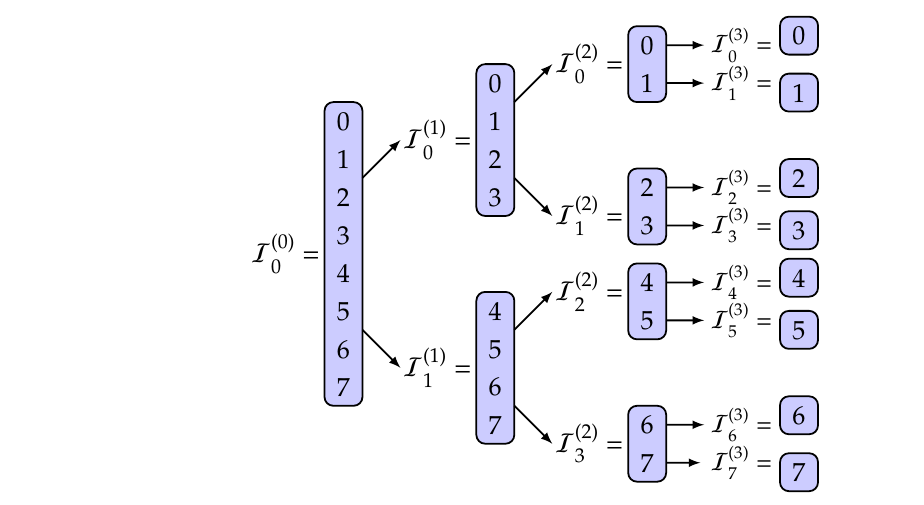
\includegraphics[scale=0.5]{1_0}
	}
	\caption{Кластерне дерево при p=3.}
	\end{figure}	

	\section{Означення блочного кластерного дерева}
	\hspace{0,8cm} Блочне кластирне дерево - це кластерне дерево над множиною індексів $I\times I$ замість $I$. В загальному, для неквадратних матриць, що належать до $\mathbb{R}^{I\times J}$, потрібно два різні cluster trees $\mathbb{T}_{I}$ та $\mathbb{T}_{J}$, тому ми розглядаємо інше cluster tree $\mathbb{T}_{J}$, яке базується на множині індексів $J$ потужності $|J|=m$. 
	\begin{Def}
	  Нехай $\mathbb{T}_{I}$ і $\mathbb{T}_{J}$ - кластерні дерева над множинами індексів $I$ та $J$ відповідно. Кластерне дерево $\mathbb{T}_{I\times J}=\mathbb{T}_{\mathbb{T}_{I}\times \mathbb{T}_{J}}=(V,E)$ називається блочним кластерним деревом над добутком множини індексів $I\times J$, якщо $\forall v\in V$ виконуються наступні умови:
	\begin{enumerate}
		\item[-] $\mathbb{T}^{(0)}_{I\times J}=I\times J$
		\item[-] Якщо $v\in \mathbb{T}^{(l)}_{I\times J}$, то існують $\tau \in \mathbb{T}^{(l)}_I$ i $\sigma \in \mathbb{T}^{(l)}_J$ такі, що $v=\tau \times \sigma$.
		\item[-] Для синів $v=\tau \times \sigma$, де  $\tau \in \mathbb{T}_I$ i $\sigma \in \mathbb{T}_J$ виконується
		\newline
		S(v)=$\begin{cases}
		$\O,$\text{якщо $S(\tau)=\O$ або $S(\sigma)=\O$}\\
		$$\{\tau^{\prime}\times\sigma^{\prime} : \tau^{\prime} \in S(\tau),\sigma^{\prime} \in S(\sigma)\}$,$\text{інакше}
		\end{cases}$
	\end{enumerate}
	\end{Def}
	\newtheorem{Th}{Теорема}[chapter]
	
	\par Властивості блочног кластирного дерева $\mathbb{T}_{I\times J}$:
	\begin{itemize}
		\item Якщо обоє клостерні дерева $\mathbb{T}_I$ i  $\mathbb{T}_J$ є бінарними деревами, то отримане блочне кластерне дерево є quad-деревом, тобто кожний внутрішній вузол має точно чотири нащадки.
		\item $|\mathcal{L}(\mathbb{T}_{I\times J})|\le |\mathcal{L}(\mathbb{T}_I)|\cdot |\mathcal{L}(\mathbb{T}_J)|$
		\item $|\mathbb{T}_{I\times J}^{(l)}|\le |\mathbb{T}_I^{(l)}|\cdot |\mathbb{T}_J^{(l)}|$
		\item $d(\mathbb{T}_{I\times J})=min\{d(\mathbb{T}_I),d(\mathbb{T}_J)\}$
	\end{itemize}
	
	\par Кількість можливих блоків $t\times s$ з вузлами $t,s$, що належать дереву $\mathbb{T}_I$ становить $(\#\mathbb{T}_I)^2=(2n-1)^2=\mathcal{O}(n^2)$. Оскільки ми не можемо тестувати всі можливі комбінації, нашою метою є зменшення квадратичної збіжності для збірки матриці. Можливим варіантом є тестування блоків рівень за рівнем починаючи від кореня $I$ дерева $\mathbb{T}_I$ і в подальшому заглиблюючись в дерево. Блоки, що тестуються, зберігають в блочному кластерному дереві $\mathbb{T}_{I\times I}$, листки якого утворюють поділ множини індексів $I\times I$. \par Алгоритм побудови блочного кластерного дерева (викликати з параметрами\newline BuildBlockClusterTree($I,I$)):
	\begin{algorithm}
	\caption{Побудова блочного кластерного дерева $\mathbb{T}_{I\times I}$}
	\begin{algorithmic}
	\STATE {\bf procedure} BuildBlockClusterTree(cluster t,s)
	\IF{$(t,s)$ is admissible}
	\STATE $S(t\times s):=\O$;
	\ELSE
	\STATE $S(t\times s):=\{t'\times s'|t'\in S(t)$ and $s'\in S(s)\}$;
	\FOR {$t'\in S(t)$ and $s'\in S(s)$}
	\STATE BuildBlockClusterTree($t',s'$);
	\ENDFOR
	\ENDIF
	\end{algorithmic}

	\end{algorithm}
	\section{Умова допустимості}
	\hspace{0.8cm} Під час побудови блочного кластерного дерева $\mathbb{T}_{I\times J}$ потрібна допоміжна умова, яка перевіряє чи блок $b=\tau\times\sigma\in \mathbb{T}_{I\times J}$ є відповідного розміру і в особливості чи він може бути наближений розрідженою матрицею. Це робиться за допомогою умови допустимості, яка в певному сенсі залежить від геометрії основної проблеми. Умова допустимості певним чином збалансовує точність апроксимації та вимоги до пам'яті $\mathcal{H}$-матриць.
	\begin{Def}
	Умова допустимості є булівською функцією 
	$$Adm:\mathbb{T}_{I\times J}\rightarrow\{true,false\}$$
	для якої виконується умова
	$$Adm(b)\Rightarrow Adm(b'),\quad\text{для всіх синів } b'\subseteq b\in \mathbb{T}_{I\times J} $$
	і властивість\newline 
	\hspace{2cm}$$Adm(b)=true, \quad\text{для всіх листків } b\in \mathbb{T}_{I\times J}$$
	\end{Def}
	\begin{Def}
		Поділ $\mathcal{P}$ називається допустимим ($\mathcal{P}_{Adm}$), якщо всі $b=(\tau\times\sigma)\in \mathcal{P}$ є допустимими.
	\end{Def}
	\hspace{0.8cm} Стандартна умова допустимості була вперше описана в класичній побудові $\mathcal{H}$-матриць, де вона застосовується для розподілу, здебільшого для проблем, що вирішуються за допомогою методу граничних елементів.
	\begin{Def}
	Нехай $\eta>0$ - фіксований параметр. Кажуть, що блок $b=\tau\times\sigma$ задовольняє стандартину умову допустимості, якщо 
	$$Adm_\eta(b)=true\Leftrightarrow min(diam(\Omega_{\tau}),diam(\Omega_{\sigma}))\le \eta\cdot dist(\Omega_{\tau},\Omega_{\sigma})$$
	де $\Omega_{\tau}$ i $\Omega_{\sigma}$ визначаються як
	$$\Omega_{\tau}:=\bigcup_{i\in \tau}supp(\varphi_i)$$
	$$\Omega_{\sigma}:=\bigcup_{i\in \sigma}supp(\varphi_i)$$
	\end{Def}
	\par В попередніх означеннях "diam" i "dist" позначають Евклідовий діаметр і відстань між $\Omega_{\tau}$ та $\Omega_{\sigma}$. Вони визначаються наступним чином:
	$$diam(\Omega_{\tau}):=\max_{x_i,x_j\in\Omega_{\tau}}||x_i-x_j||$$
	$$dist(\Omega_{\tau},\Omega_{\sigma}):=\min_{x_i\in\Omega_{\tau},x_j\in\Omega_{\sigma}}||x_i-x_j||$$
	\par Якщо в означені 4.3 замінити "min" на "max", то отримуємо сильну умову допустимості:
	$$Adm_\eta(b)=true\Leftrightarrow max(diam(\Omega_{\tau}),diam(\Omega_{\sigma}))\le \eta\cdot dist(\Omega_{\tau},\Omega_{\sigma})$$
	\par В подальшому для одновимірної проблеми ми будемо використовувати стандартну умову допустимості в такому вигляді
	\newline
	$$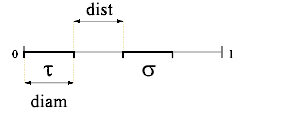
\includegraphics{1_2}$$
	$$diam(\tau)\le dist(\tau,\sigma)$$
	\begin{Def}
		Блок індексів $t\times s\subset I\times I$ називається допустимим, якщо відповідна область $\tau\times\sigma$ з $\tau:=\bigcup_{i\in t}supp\varphi_i,\sigma:=\bigcup_{i\in s}supp\varphi_i$ задовільняє умову 
		$$diam(\tau)\le dist(\tau,\sigma)$$
	\end{Def}

	\section{Означення $\mathcal{H}$-матриці}
	\hspace{0.8cm} На допустимих блоках апроксимуємо за допомогою структури rkmatrix. На недопустимих листках використовуємо структуру fullmatrix.
	\par $n_{min}$ - розмірність найменшого листка.
	\begin{Def}
	Нехай $M\in\mathbb{R}^{I\times J}$ - матриця над множиною індексів $I\times J$. Підматриця $(M_{i,j})_{(i,j)\in I'\times J'}$ для підмножини $I'\times J'$ множини $I\times J$ позначається як $M|_{I'\times J'}$.
	\end{Def}
	\begin{Def}
	($\mathcal{H}$-матриця) Нехай $k,n_{min}\in \mathbb{N}_0$. Множина $\mathcal{H}$-матриць, що базується на допустимому поділі $\mathcal{P}_{Adm}$ над блочним кластерним деревом $\mathbb{T}:=\mathbb{T}_{I\times J}$ визначається як 
	$$\mathcal{H}(\mathbb{T},k):=\{M\in\mathbb{R}^{I\times J}|\forall\tau\times\sigma\in\mathcal{P}_{Adm}:rank(M|_{\tau\times\sigma})\le k \text{ або } \min(|\tau|,|\sigma|)\le n_{min} \}$$ 
	\end{Def}
	\par Спрощене означення $\mathcal{H}$-матриці виглядає наступним чином 
	\begin{Def}
	Нехай $\mathbb{T}_{I\times I}$ - блочне кластерне дерево над множиною індексів $I$. Означаємо множину $\mathcal{H}$-матриць як
	$$\mathcal{H}(\mathbb{T}_{I\times I},k):=\{M\in\mathbb{R}^{I\times I}|rank(M|_{t\times s})\le k \text{ для всіх допустимих листків } t\times s \text{ дерева } \mathbb{T}_{I\times I} \}$$
	\end{Def}
	\section{Приклад побудови блочного кластерного дерева.}
	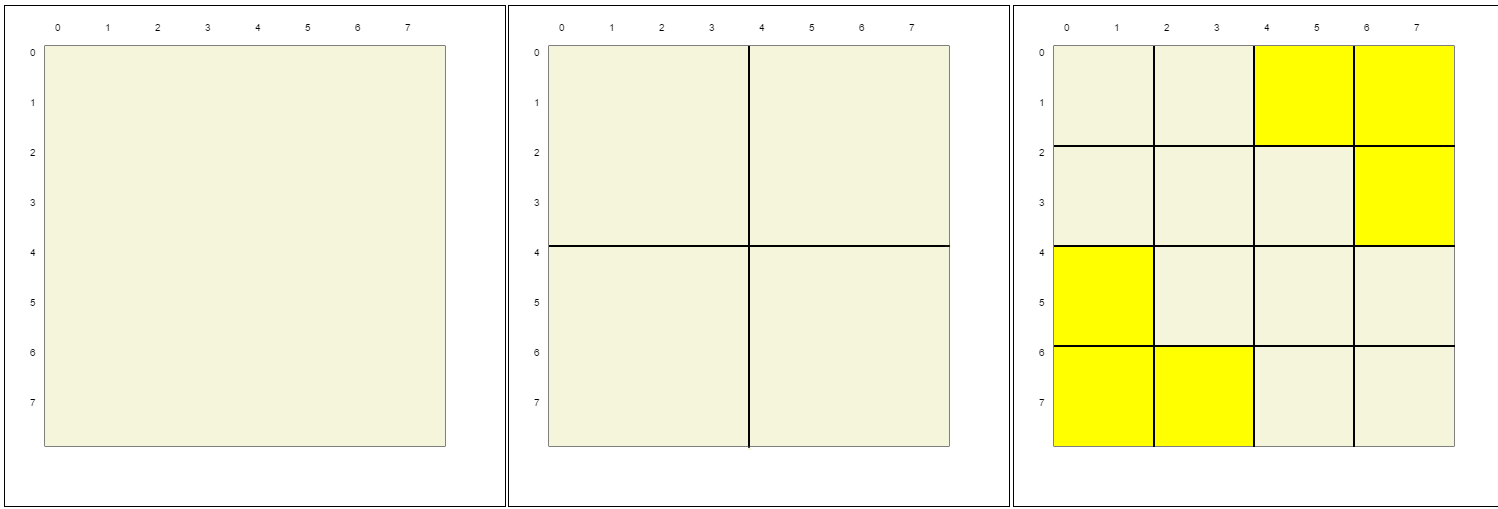
\includegraphics[scale=0.45]{1_3}
	\par Кроки побудови блочного кластерного дерева при p=3:
	\begin{enumerate}
	\item Коренем дерева є блок $\{0,1,2,3,4,5,6,7\}\times\{0,1,2,3,4,5,6,7\}$, який не задовільняє умову допустимості, тому що відповідною областю до множини індексів $\{0,1,2,3,4,5,6,7\}$ є інтервал $[0,1]$ i $$diam([0,1])=1\le 0=dist([0,1],[0,1])$$
	\item Чотирьма нащадками кореня в дереві $\mathbb{T}_{I\times I}$ є
	$$\{0,1,2,3\}\times\{0,1,2,3\},\quad\{0,1,2,3\}\times\{4,5,6,7\},$$
	$$\{4,5,6,7\}\times\{0,1,2,3\},\quad\{4,5,6,7\}\times\{4,5,6,7\}.$$
	\par Жоден з них не задовільняє умову допустимості.
	\item Після подальшого поділу, отримуємо такі блоки:
	$$\{0,1\}\times\{0,1\},\quad\{0,1\}\times\{2,3\},\quad\{0,1\}\times\{4,5\},\quad\{0,1\}\times\{6,7\},$$
	$$\{2,3\}\times\{0,1\},\quad\{2,3\}\times\{2,3\},\quad\{2,3\}\times\{4,5\},\quad\{2,3\}\times\{6,7\},$$
	$$\{4,5\}\times\{0,1\},\quad\{4,5\}\times\{2,3\},\quad\{4,5\}\times\{4,5\},\quad\{4,5\}\times\{6,7\},$$
	$$\{6,7\}\times\{0,1\},\quad\{6,7\}\times\{2,3\},\quad\{6,7\}\times\{4,5\},\quad\{6,7\}\times\{6,7\}.$$
	Деякі з циз вузлів задовольняють умову допустимості, наприклад вузол $\{0,1\}\times\{4,5\}$, тому що відповідною областю є $[0,\frac{1}{4}]\times [\frac{1}{2},\frac{3}{4}]$:
	$$diam([0,\frac{1}{4}])=\frac{1}{4}=dist([0,\frac{1}{4}],[\frac{1}{2},\frac{3}{4}])$$
	Вузли на діагоналі не задовольняють умову допустимості (відстань від відповідної області до себе самої рівна нулю) і деякі вузли не на діагоналі (наприклад $\{0,1\}\times \{2,3\}$) не задовольняють умову допустимості.
	\item Нащадками цих вузлів є $\{(i,j)\}$ для індексів $i,j$. 
	Кінцева структура буде:
	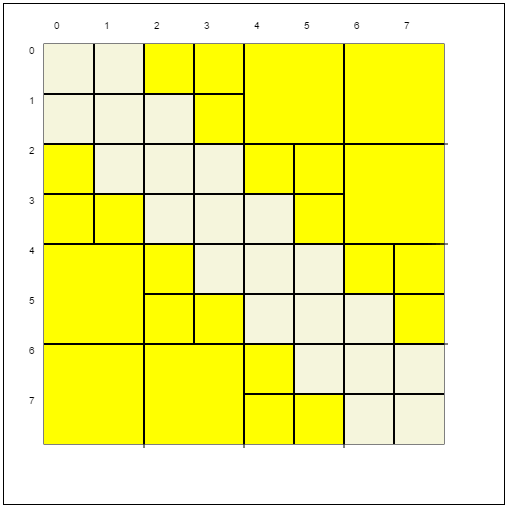
\includegraphics[scale=0.5]{1_4}
	\end{enumerate}
	\par Аналогічно можна побудувати блочного кластерного дерева для $p=4$ чи $p=5$.
	\chapter{3. Розв'язання модельного інтегрального рівняння.}
	\section{Модельна задача}
	\hspace{0.8cm}Розглянемо застосування {$\mathcal{H}$}-матриць на прикладі одновимірного інтегрального рівняння Фредгольма першого роду. Нехай задано функцію $F:[0,1]\rightarrow \mathbb{R}$. Шукаємо функцію $u:[0,1]\rightarrow \mathbb{R}$, яка задовільняє наступне інтегральне рівняння: $$\int_{0}^{1}\ln|x-y|u(y)dy=F(x), x\in[0,1]$$
	де $g(x,y)=\ln|x-y|$ називається ядром інтегрального рівняння і має невизначеність на діагоналі $x=y$.
	\par Використовуючи метод Гальоркіна,проектуємо дане рівнання на n-вимірний простір $V_n=span\{\varphi_0,\dots,\varphi_{n-1}\}$
	i отримуємо:
	$$\int_{0}^{1}\int_{0}^{1}\varphi_i(x)\ln|x-y|u(y)dydx=\int_{0}^{1}\varphi_i(x)F(x)dx$$
	$0\le i<n$
	\par Потрібно знайти $u_n$ в просторі $V_n$:
	$$u_n=\sum_{j=0}^{n-1}u_j\varphi_j$$
	таке, що вектор коефіцієнтів $u$ є розв'язком лінійної системи $$Gu=f$$
	$$G_{ij}=\int_{0}^{1}\int_{0}^{1}\varphi_i(x)\ln|x-y|\varphi_j(y)dydx$$
	$$f_i=\int_{0}^{1}\varphi_i(x)F(x)dx$$
	 В цьому прикладі визначаємо базисні функції як
	\newline 
	\begin{equation*}
	\varphi_i(x)=\begin{cases}
			1,\quad\text{якщо $\frac{i}{n}\le x\le \frac{i+1}{n}$}\\
			0,\quad\text{інакше}
				\end{cases}
	\end{equation*}
	\newline
	які в загальному матимуть вигляд 
	\newline
		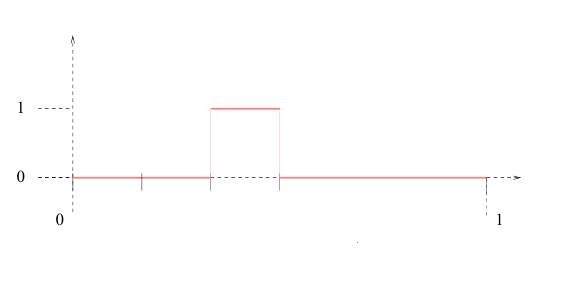
\includegraphics{1_1}
	\par Матриця G є щільною, тобто всі елементи не є нулями. Потрібно знайти наближену матрицю \~G, яка може бути збереженою в розрідженому форматі. Для того, щоб це досягти потрібно замінити ядро $g(x,y)=\ln|x-y|$ на розкладене ядро $$\tilde{g}(x,y)=\sum_{v=0}^{k-1}g_v(x)h_v(y)$$
	\par Таким чином, інтегрування за змінною x буде відкремленим від інтегрування за змінною y. Проте, ядро  $g(x,y)=\ln|x-y|$ не можна наблизити розкладеним ядром на цілій області $[0,1]\times[0,1]$ (хіба що при великому k). Змість цього, ми будуємо локальні наближення на підобластях $[0,1]\times[0,1]$, де $g$ є гладкою.
	\section{Розклад ядра в ряд Тейлора}
	\hspace{0.8cm}Нехай $\tau:=[a,b]$, $\sigma:=[c,d]$, $\tau\times\sigma\subset[0,1]\times[0,1]$ буде підобластю з властивістю $b<c$ і інтервали є роз'єднаними, тобто $$\tau\cap\sigma=\O$$
	Тоді ядро є визначеним на $\tau\times\sigma$. $x_0:=(a+b)/2$
	\newtheorem{Lem}{Лема}[chapter]
	\begin{Lem}
		{\bf (Похідні $\ln|x-y|$)} Похідні $g(x,y)=\ln|x-y|$ для $x\not=y$ i $v\in \mathbb{N}$ мають вигляд
		$$\partial^v_xg(x,y)=(-1)^{v-1}(v-1)!(x-y)^{-v}$$
		$$\partial^v_yg(x,y)=(v-1)!(x-y)^{-v}$$
	\end{Lem}
	\begin{Lem}
	{\bf (Розклад Тейлора для $\ln|x-y|$)} Для будь-якого $k\in \mathbb{N}$ функція 
	$$\tilde{g}(x,y)=\sum_{v=0}^{k-1}\frac{1}{v!}\partial^v_xg(x_0,y)(x-x_0)^v$$
	наближає ядро $g(x,y)=\ln|x-y|$ з похибкою
	$$|g(x,y)-\tilde{g}(x,y)|\le(1+\frac{|x_0-a|}{|c-b|})(1+\frac{|c-b|}{|x_0-a|})^{-k}$$
	\end{Lem}
	 Доведення. Нехай $x\in [a,b],a<b$ i $y\in [c,d]$. В радіусі збіжностi ряд Тейлора для ядра $g(x,y)$ в точці $x_0$ задовільняє $$g(x,y)=\sum_{v=0}^{\infty}\frac{1}{v!}\partial^v_xg(x_0,y)(x-x_0)^v$$
	Залишок $g(x,y)-\tilde{g}(x,y)=\sum_{v=k}^{\infty}\frac{1}{v!}\partial^v_xg(x_0,y)(x-x_0)^v$ може бути оцінений як:
	$$|\sum_{v=k}^{\infty}\frac{1}{v!}\partial^v_xg(x_0,y)(x-x_0)^v|= |\sum_{v=k}^{\infty}(-1)^{v-1}\frac{(v-1)!}{v!}\genfrac{(}{)}{1pt}{0}{x-x_0}{x_0-y}^v|$$
	$$\le \sum_{v=k}^{\infty}|\frac{x-x_0}{x_0-y}|^v\le\sum_{v=k}^{\infty}\genfrac{(}{)}{1pt}{0}{|x_0-a|}{|x_0-a|+|c-b|}^v $$
	$$=(1+\frac{|x_0-a|}{|c-b|})(1+\frac{|c-b|}{|x_0-a|})^{-k}$$
	\newline Радіус збіжності покриває весь інтервал $[a,b]$. 
	\newline
	\par Якщо $c\rightarrow b$, то оцінка залишку прямує до нескінченості і наближення буде як завгодно поганим. Проте, якщо замінити умову $b<c$ (диз'юнкція інтервалів) сильнішою умовою допустимості
	$$diam(\tau)\le dist(\tau,\sigma)$$
	то похибка апроксимації може бути оцінена як 
	$$|g(x,y)-\tilde{g}(x,y)|\le\frac{3}{2}(1+\frac{2}{1})^{-k}=\frac{3}{2}3^{-k}$$
	\par Це означає, що ми отримуємо рівномірну оцінку для похибки наближення незалежно від інтервалів, якщо умова допустимості виконується. Похибка зростає експоненціально в залежності від порядку $k$.
	\section{Наближення низького рангу блоків матриці}
	\par Множина індексів $I=\{0,1,\dots,n-1\}$ містить індекси базових функцій $\varphi_i$, які використовуються в дискритизації Галеркіна. Фіксуємо дві підмножини $t$ і $s$ множини індексів $I$ та визначимо відповідні області:
	$$\tau=\bigcup_{i\in t}supp(\varphi_i)$$
	$$\sigma=\bigcup_{i\in s}supp(\varphi_i)$$
	\par Якщо $\tau\times\sigma$ задовільняє умову допустимості, то ми можемо наблизити ядро $g$ в цій підобласті рядом Тейлора $\tilde{g}$ і замінити елементи матриці
	$$G_{ij}=\int_{0}^{1}\int_{0}^{1}\varphi_i(x)g(x,y)\varphi_j(y)dydx$$
	використовуючи вироджене ядро $\tilde{g}=\sum_{v=0}^{k-1}g_v(x)h_v(y)$ для індексів $(i,j)\in t\times s$:
	$$\tilde{G}_{ij}=\int_{0}^{1}\int_{0}^{1}\varphi_i(x)\tilde{g}(x,y)\varphi_j(y)dydx$$
	Розділяємо подвійний інтеграл на два звичайні
	$$\tilde{G}_{ij}=\int_{0}^{1}\int_{0}^{1}\varphi_i(x)\sum_{v=0}^{k-1}g_v(x)h_v(y)\varphi_j(y)dydx $$
	$$=\sum_{v=0}^{k-1}(\int_{0}^{1}\varphi_i(x)g_v(x)dx)(\int_{0}^{1}\varphi_j(y)h_v(y)dy)$$
	\par Підматриця $G|_{t\times s}$ може бути записана в факторизованій формі
	$$G|_{t\times s}=AB^\top,\quad A\in\mathbb{R}^{t\times\{0,\dots,k-1\}},\quad B\in\mathbb{R}^{s\times\{0,\dots,k-1\}}$$
	де елементами матиць $A$ i $B$  
	$$A_{iv}:=\int_{0}^{1}\varphi_i(x)g_v(x)dx, \quad B_{jv}:=\int_{0}^{1}\varphi_j(y)h_v(y)dy$$
	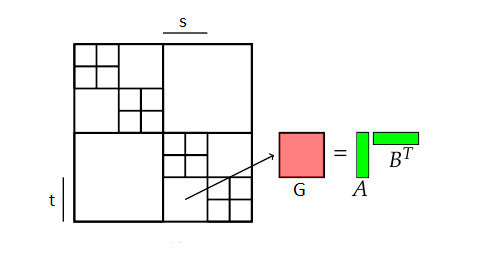
\includegraphics{1_6}
	\par Матриця $AB^\top$ має найбільший ранг $k$ в незалежності від потужності $s$ i $t$. Похибка наближення блоку матриці оцінена в наступній лемі.
	\begin{Lem}
	Поелементна похибка для елементів матриці $G_{ij}$ апроксимується ядром $\tilde{g}$ в допустимих блоках $t\times s$ ($g$ в інших блоках) обмежена наступним чином
	$$|G_{ij}-\tilde{G}_{ij}|\le \frac{3}{2}n^{-2}3^{-k}$$
	\end{Lem}
	{\bf Доведення.} $\quad|G_{ij}-\tilde{G}_{ij}|=|\int_{0}^{1}\int_{0}^{1}\varphi_i(x)(g(x,y)-\tilde{g}(x,y)\varphi_j(y)dydx|$
	$$\le \int_{0}^{1}\int_{0}^{1}|\varphi_i(x)|\frac{3}{2}3^{-k}|\varphi_j(y)|dydx$$
	$$=\frac{3}{2}3^{-k}\int_{0}^{1}\varphi_i(x)dx\int_{0}^{1}\varphi_j(y)dy$$
	$$= \frac{3}{2}n^{-2}3^{-k} \quad\blacksquare$$ 
	\par Припустимо, що ми поділили множину індексів $I\times I$ над матрицею $G$ на допустимі блоки, де застосовується апроксимація низького рангу, і недопустимі блоки, де використовуємо елементи матриці $G$.
	$$I\times I=\bigcup_{v=1,\dots,b}t_v\times s_v$$
	\par Глобальну похибку наближення оцінюємо, застосовуючи норму Фробеніуса 
	$$\|M\|^2_F:=\sum M_{ij}^2$$
	\begin{Lem}
	Похибка наближення $\|G-\tilde{G}\|_F$ для матриці $\tilde{G}$, побудованої за допомогою ядра $\tilde{g}$ в допустимих блоках $t_v\times s_v$ та з допомогою $g$ на недопустимих блоках, обмежена наступним чином
	$$\|G-\tilde{G}\|_F\le \frac{3}{2}n^{-1}3^{-k}$$
	\end{Lem}
	\par Постає питання, як поділити множину індексів $I\times I$ на допустимі та недопустимі блоки. Тривіальним поділом був би $\mathcal{P}:=\{(i,j)|i\in I,j\in I\}$, де є тільки блоки розмірності $1\times 1$, ранг рівний 1. В цьому випадку, матриця $\tilde{G}$ є ідентичною до $G$, але в цьому випадку ми не апроксимуємо матрицю у великих підблоках матрицями низького рангу. 
	\section{Побудова матриці}
	\hspace{0.8cm} Ієрархічна матриця розкладається на допустимі і недопустимі листки дерева $\mathbb{T}_{I\times I}$. Для них створені два підкласи, опрацювання яких різниться.
	\subsection{Недопустимі листки}
	\hspace{0.8cm} В недопустимих, але малих блоках $t\times s\subset I\times I$ обчислюємо елементи матриці $(i,j)$ за формулою
	$$\tilde{G_{ij}}:=\int_{0}^{1}\int_{0}^{1}\varphi_i(x)\ln|x-y|\varphi_j(y)dydx$$$$=\int_{i/n}^{(i+1)/n}\int_{j/n}^{(j+1)/n}\ln|x-y|dydx$$
	\begin{Def}
		(репрезентація fullmatrix) Кажуть, що матриця $M$ розмірності $n\times m$ зберігається у вигляді fullmatrix, якщо її елементи $M_{ij}$ зберігаються як дійсні числа у масиві довжиною $mn$ в стовпцевому порядку
		$$M_{11},\dots,M_{n1},M_{12},\dots,M_{n2},\dots,M_{1m},\dots,M_{nm}$$
	\end{Def}
	\par Порядок елементів матриці в репрезентації fullmatrix є таким самим, як і в стандартних пакетах лінійної алгебри (MATLAB,BLAS,LAPACK тощо).
	\par Реалізація на мові програмування $C\#$:
	\begin{verbatim}
	public class Fullmatrix
	    {
	        public int rows;
	        public int cols;
	        public double[] e;
	    }
	\end{verbatim}
	\subsection{Допустимі листки}
	\hspace{0.8cm} В допустимих блоках $t\times s\subset I\times I$ з відповідними областями $[a,b]\times [c,d]$ i $x_0:=(a+b)/2$ обчислюємо відповідну матрицю у факторизованій формі
	$$\tilde{G}|_{t\times s}:=AB^\top$$
	$$A_{iv}:=\int_{i/n}^{(i+1)/n}(x-x_0)^vdx$$
	\begin{equation*}
		B_{jv}:=\begin{cases}
					(-1)^{v+1}v^{-1}\int_{j/n}^{(j+1)/n}(x_0-y)^{-v}dy,\quad\text{якщо $v>0$}\\
					\int_{j/n}^{(j+1)/n}\ln|x_0-y|dy,\quad\text{якщо $v=0$}
				\end{cases}
	\end{equation*}
	\par Підходящою репрезентацією для відповідної матриці $\tilde{G}|_{t\times s}$ є формат rkmatrix наведений нище.
	\begin{Def}
		(репрезентація rkmatrix)  Кажуть, що матриця $M$ розмірності $n\times m$ найбільшого рангу $k$ зберігається у вигляді rkmatrix, якщо вона зберігається у факторизованій формі $M=AB^\top$, де обидві матриці $A\in\mathbb{R}^{n\times k}$ i $B\in \mathbb{R}^{m\times k}$ зберігаються як масиви (в стовпцевому порядку).
	\end{Def}
	\par Реалізація на мові програмування $C\#$:
	\begin{verbatim}
	public class Rkmatrix
	    {
	        public int k;
	        public int rows;
	        public int cols;
	        public double[] a;
	        public double[] b;
	    }
	\end{verbatim}
	\subsection{Репрезентація ієрархічної матриці}
	\begin{Def}
		(репрезентація $\mathcal{H}$-матриці)  Нехай $\mathbb{T}_{I\times I}$ - блочне кластерне дерево над множиною індексів $I$. Кажуть, що матриця $M\in\mathcal{H}(\mathbb{T}_{I\times I},k)$ зберігається в $\mathcal{H}$-matrix репрезентації, якщо підматриці, що відповідають недопустимим листкам, зберігаються у вигляді fullmatrix, а ті, що відповідають допустимим листкам - у вигляді rkmatrix. 
	\end{Def}
	\par Однією можливою реалізацією $\mathcal{H}$-matrix репрезентації є зберігання допустимих і недопустимих блоків матриці в списку. Збірка і множення матриці на вектор робиться для кожного блоку окремо. Проте, ми використаємо іншу реалізацію, яка базується на структурі block cluster tree $\mathbb{T}_{I\times I}$ (не тільки на листках) і таким чином зберігає матрицю у більш структурованому вигляді.
	\par Кожен блок $t\times s$ в дереві $\mathbb{T}_{I\times I}$ може бути 
	\begin{itemize}
		\item листком - тоді відповідний блок матриці представлений у вигляді fullmatrix або rkmatrix.
		\item не листком - тоді блок $t\times s$ розкладають на його синів $t'\times s'$ з $t'\in S(t)$ та $s' \in S(s)$. Це означає матриця, що відповідає блоку $t\times s$ -- $supermatrix$ і вона складається з підматриць, що відповідають блоку $t'\times s'$.
	\end{itemize} 
	\par Реалізація на мові програмування $C\#$:
	\begin{verbatim}
	public class Supermatrix
	    {
	        public int rows;
	        public int cols;
	        public int blockrows;
	        public int blockcols;
	        public Rkmatrix r;
	        public Fullmatrix f;
	        public Supermatrix[,] s;
	    }
	\end{verbatim}

	$$M\in\mathbb{R}^{rows\times cols}$$
	\par Матриця може бути 
	\begin{itemize}
		\item rkmatrix - тоді 
		$$r\not=null,\quad
		f=null,\quad
		s=null$$
		Матриця $r$ - це репрезентація rkmatrix матриці $M$.
		\item fullmatrix - тоді  
		$$r=null,\quad
		f\not=null,\quad
		s=null$$
		Матриця $f$ - це репрезентація fullmatrix матриці $M$.
		\item supermatrix - тоді
		$$r=null,\quad
		f=null,\quad
		s\not=null$$
		Матриця $s$ містить вказівники на підматриці $M_{i,j}$:
		\[
			\begin{pmatrix}
				M_{1,1} & \dots & M_{1,blockcols}\\
				\vdots & \ddots & \vdots \\
				M_{blockrows,1} &\dots  & M_{blockrows,blockcols}
			\end{pmatrix}
		\]
		в порядку 
		$$M_{1,1},\dots,M_{blockrows,1},M_{1,2},\dots,M_{blockrows,2},\dots,M_{1,blockcols},\dots,M_{blockrows,blockcols}$$
	\end{itemize}
	\par Реалізацією $\mathcal{H}$-матриці є дерево з вузлами, що реалізовані як $supermatrix$. На додаток, структура таж сама, що і в блочному кластерному дереві $\mathbb{T}_{I\times I}$ (нащадки $\equiv$ підматриці) і підматриці, що відповідають допустимим та недопустимим листкам, зберігаються в форматі rkmatrix i fullmatrix.
	\section{Метод спряжених градієнтів}
	\par Метод спряжених градієнтів (conjugate gradient method) - це алгоритм для чисельного розв'язування певних систем лінійних рівнянь, особливо тих в яких матриця є симетричною і додатньо визначеною. Часто релізують як ітераційний алгоритм, що застосовується до розріджених систем, які завеликі для розв'язування прямими методами (наприклад з допомогою методу Холецького).
	\par Метод спряжених градієнтів вимагає від матриці тільки можливості помножити її на вектор, що дає можливість застосовувати спеціальні формати зберігання матриці.
	\begin{algorithm}
	\caption{Алгоритм методу спряжених градієнтів}
	\begin{algorithmic}
		\STATE $r_0:=b-Ax$
		\STATE $p_0:=r_0$
		\STATE $k:=0$
		\WHILE {$true$}
			\STATE $\alpha_k:=\frac{r_k^{\intercal}r_k}{p_k^{\intercal}Ap_k}$
			\STATE $x_{k+1}:=x_k+\alpha_kp_k$
			\STATE $r_{k+1}:=r_k-\alpha_kAp_k$
			\IF {$r_{k+1}$ достатньо мале}
				\STATE вийти з циклу
			\ENDIF
			\STATE $\beta_k=\frac{r_{k+1}^{\intercal}r_{k+1}}{r_k^\intercal r_k}$
			\STATE $p_{k+1}:=r_{k+1}+\beta_kp_k$
			\STATE $k:=k+1$
		\ENDWHILE
		\STATE результатом є $x_{k+1}$
	\end{algorithmic}
	
	\end{algorithm}
	\section{Програмна реалізація}
	\hspace{0.8cm} Програмна реалізація на мові $С\#$ в стані доробки. Працюють такі описані у роботі алгоритмів(код в додатках):
		 \begin{enumerate}
		 	\item побудова cluster tree для $n=2^p$.
		 	\item побудова block cluster tree.
		 	\item множення $\mathcal{H}-$матриці на вектор.
		 	\item реалізація методу спряжених градієнтів.
		 \end{enumerate}
	\begin{figure}[bh]\centering{
			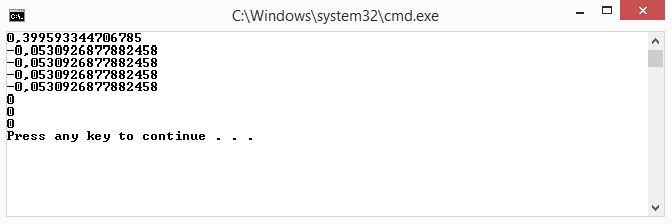
\includegraphics[scale=0.65]{1_8}
			}
			\caption{Реалізація BEM.}	 
			\end{figure}
	\chapter{4. Розв'язання задачі Діріхле для рівняння Лапласа на площині}
	\chapter{Висновок}
	\hspace{0.8cm} В цій роботі розглянуто основні принципи побудови та використання $\mathcal{H}$-матриць. Описано такі ключові поняття як дерево, кластерне дерево та блочне кластерне дерево, які лягли в основу означення структури ієрархічної матриці. Також розглянуто відповідні структури через які ієрархічні матриці реалізують програмно: rkmatrix, fullmatrix та supermatrix. Наведено алгоритми реалізації блочного кластерного дерева i методу спряжених градієнтів.
	\par Застосування $\mathcal{H}$-матриць розглянуто на прикладі методу скінченних елементів (BEM). У даному прикладі застосовується метод Галеркіна та метод спряжених градієнтів. 
	\chapter{Додатки}
	\begin{enumerate}
		\item Побудова Cluster Tree
		
			\begin{verbatim}
			 public static ClusterTree buildClusterTreeRec(int b, int e, int level,
			  int num, int[] arr)
			        {
			            ClusterTree t = new ClusterTree();
			            t.level = level;
			            t.numberOfLeaf = num;
			            int n = e - b + 1;
			            t.leaf = new int[n];
			            for (int i = 0; i < t.leaf.Length; i++)
			                t.leaf[i] = i + b;
			            int m = (int)Math.Pow(2, level) - arr[level];
			            arr[level]--;
			            if (n != 1)
			            {
			                t.leftTree = buildClusterTreeRec(b, (b + e + 1) / 2 - 1,
			                    level + 1, m, arr);
			                m = (int)Math.Pow(2, level) - arr[level];
			                arr[level]--;
			                t.rightTree = buildClusterTreeRec((b + e + 1) / 2, e,
			                    level + 1, m, arr);
			            }
			            else
			            {
			                t.leftTree = null;
			                t.rightTree = null;
			            }
			            return t;
			        }
			\end{verbatim}
		\item Побудова Block Cluster Tree
		\begin{verbatim}
		public static Supermatrix BuildBlockClusterTree(ClusterTree t,ClusterTree s,
		    Supermatrix spr,int n)
		        {
		            if (IsAdmissible(t, s))
		            {
		                spr.s = null;
		                spr.r = new Rkmatrix();
		                spr.r.rows = t.leaf.Length;
		                spr.r.cols = s.leaf.Length;
		                spr.r.k = spr.r.rows;
		                spr.r.a = new double[spr.r.rows * spr.r.cols];
		                spr.r.b = new double[spr.r.rows * spr.r.cols];
		                FillRkmatrix(t,s,out spr.r.a,out spr.r.b);
		                return spr;
		             }
		             else
		             {
		                if (t.leaf.Length != 1)
		                {
		                   spr.rows = n;
		                   spr.cols = n;
		                   spr.blockrows = 2;
		                   spr.blockcols = 2;
		                   spr.s = new Supermatrix[spr.blockrows, spr.blockcols];
		                   for (int i = 0; i < spr.s.GetLength(0); i++)
		                   {
		                       for (int j = 0; j < spr.s.GetLength(1); j++)
		                          spr.s[i, j] = new Supermatrix();
		                   }
		                   spr.s[0, 0] = BuildBlockClusterTree(t.leftTree,
		                           s.leftTree, spr.s[0, 0],n);
		                   spr.s[0, 1] = BuildBlockClusterTree(t.rightTree,
		                           s.leftTree, spr.s[0, 1],n);
		                   spr.s[1, 0] = BuildBlockClusterTree(t.leftTree,
		                           s.rightTree, spr.s[1, 0],n);
		                   spr.s[1, 1] = BuildBlockClusterTree(t.rightTree,
		                           s.rightTree, spr.s[1, 1],n);
		               }
		               else
		               {
		               	   spr.rows = n;  spr.cols = n;
		                   spr.s = null;
		                   spr.f = new Fullmatrix();
		                   spr.f.cols = 0;	  spr.f.rows = 0;
		                   FillFullmatrix(t,s,out spr.f.e);
		               }
		            return spr;
		         }
		                
		\end{verbatim}
		\item Множення $\mathcal{H}$-матриці на вектор
		\begin{verbatim}
		static public double[] MultHMatrixByVector(Supermatrix spr, double[] vct)
		        {
		            if (spr.s != null)
		            {
		                int n=vct.Length;
		                double[] vct1=new double[(int)(n/2)];
		                double[] vct2=new double[(int)(n/2)];
		                for (int i=0;i<n/2;i++){
		                    vct1[i]=vct[i];
		                    vct2[i]=vct[i+(int)(n/2)];
		                }
		                double[] a1=MultHMatrixByVector(spr.s[0, 0], vct1);
		                double[] a2=MultHMatrixByVector(spr.s[0, 1], vct2);
		                double[] b1=MultHMatrixByVector(spr.s[1, 0], vct1);
		                double[] b2=MultHMatrixByVector(spr.s[1, 1], vct2);
		                double[] res = new double[n];
		                for (int i = 0; i < (int)n / 2; i++)
		                {
		                    res[i] = a1[i] + a2[i];
		                    res[i + (int)n / 2] = b1[i] + b2[i];
		                }
		                return res;
		            }
		            else
		            {
		                if (spr.r != null)
		                {
		                    double[,] tempa=new double[spr.r.rows,spr.r.cols];
		                    double[,] tempb=new double[spr.r.rows,spr.r.cols];
		                    int k = 0;
		                    for (int i = 0; i < spr.r.rows; i++)
		                    {
		                        for (int j = 0; j < spr.r.cols; j++)
		                        {
		                            tempa[i, j] = spr.r.a[k];
		                            tempb[i, j] = spr.r.b[k];
		                            k++;
		                        }
		                    }
		                    double[] first = GradientMethod.
		                        MultiplyMatrixByVector(tempb, vct);
		                    double[] second = GradientMethod.
		                        MultiplyMatrixByVector(tempa, first);
		                    return second;
		                }
		                else if (spr.f != null)
		                {
		                    double[] res = new double[1];
		                    res[0]=GradientMethod.MultiplyVectorByVector(spr.f.e, vct);
		                    return res;
		                }
		            }
		     }
		\end{verbatim}
		\item Реалізація алгоритму методу спряжених градієнтів
		\begin{verbatim}
		public static double[] ConjugateGradientMethodHMatrix(Supermatrix a, 
				double[] b, double[] x0)
		        {
		            int n = b.Length;
		            double[] x1 = new double[n];
		            double[] temp = BlockClusterTree.MultHMatrixByVector(a, x0);
		            double[] r0 = new double[n];
		            double[] p0 = new double[n];
		            double[] r1 = new double[n];
		            double[] p1 = new double[n];
		            double alphak = 0;
		            double betak = 0;
		            for (int i = 0; i < n; i++)
		                r0[i] = b[i] - temp[i];
		            p0 = r0;
		            int k = 0;
		            while (k != n)
		            {
		                double temp1 = MultiplyVectorByVector(r0, r0);
		                double[] temp2 = BlockClusterTree.MultHMatrixByVector(a, p0);
		                double temp3 = MultiplyVectorByVector(temp2, p0);
		                alphak = temp1 / temp3;
		                for (int i = 0; i < n; i++)
		                {
		                    x1[i] = x0[i] + alphak * p0[i];
		                    r1[i] = r0[i] - alphak * temp2[i];
		                }
		                betak = MultiplyVectorByVector(r1, r1) /
		                	 MultiplyVectorByVector(r0, r0);
		                for (int i = 0; i < n; i++)
		                    p1[i] = r1[i] + betak * p0[i];
		                p0 = p1;
		                r0 = r1;
		                x0 = x1;
		                k++;
		            }
		            return x1;
		        }
		\end{verbatim}
	\end{enumerate}
	\newpage
	\begin{thebibliography}{00}
	\normalsize{
		\bibitem{HM}
	    	Steffen B\"orm {\it Hierarchical Matrices} / Lars Grasedyck, Wolfgang Hackbusch --- електронний ресурс, 2005. --- 136 c.
		\bibitem{Diss}
			Mohammad Izadi {\it Hierarchical Matrix Techniques on Massively Parallel Computers. Dissertation}---K.: Max Planck Institute for Mathematics in the Sciences,2012.--- 212 c.
		\bibitem{Descrete}
			Нікольський Ю.В. {\it Дискретна математика} / Пасічник В.В., Щербина Ю.М.---К.: Видавнича група BHV,2007.---368 c.
		\bibitem{Wolfg}
			 Wolfgang Hackbusch {\it Hierarchical Matrices: Algorithms and Analysis}---K.: Springer-Verlag,2015.--- 505 c.
		
		\bibitem{fghj}
			Lin Lin {\it Fast construction of hierarchical matrix representation from matrix–vector
			multiplication } /  Jianfeng Lu, Lexing Ying --- K.: Journal of Computational Physics 230 4071–4087,2011.---17 c.
		\bibitem{Gradient}
			Jonathan Richard Shewchuk {\it An Introduction to the Conjugate Gradient Method Without the Agonizing Pain }---K.:School of Computer Science, Pittsburg,PA 15213,1994.---64 c. 	 
	}
	\end{thebibliography}	
\end{document}